\documentclass[tikz, border=7pt]{standalone}

\usepackage{tikz}
\usetikzlibrary{positioning,shadows,arrows}

\usepackage[T1]{fontenc}

\begin{document}
    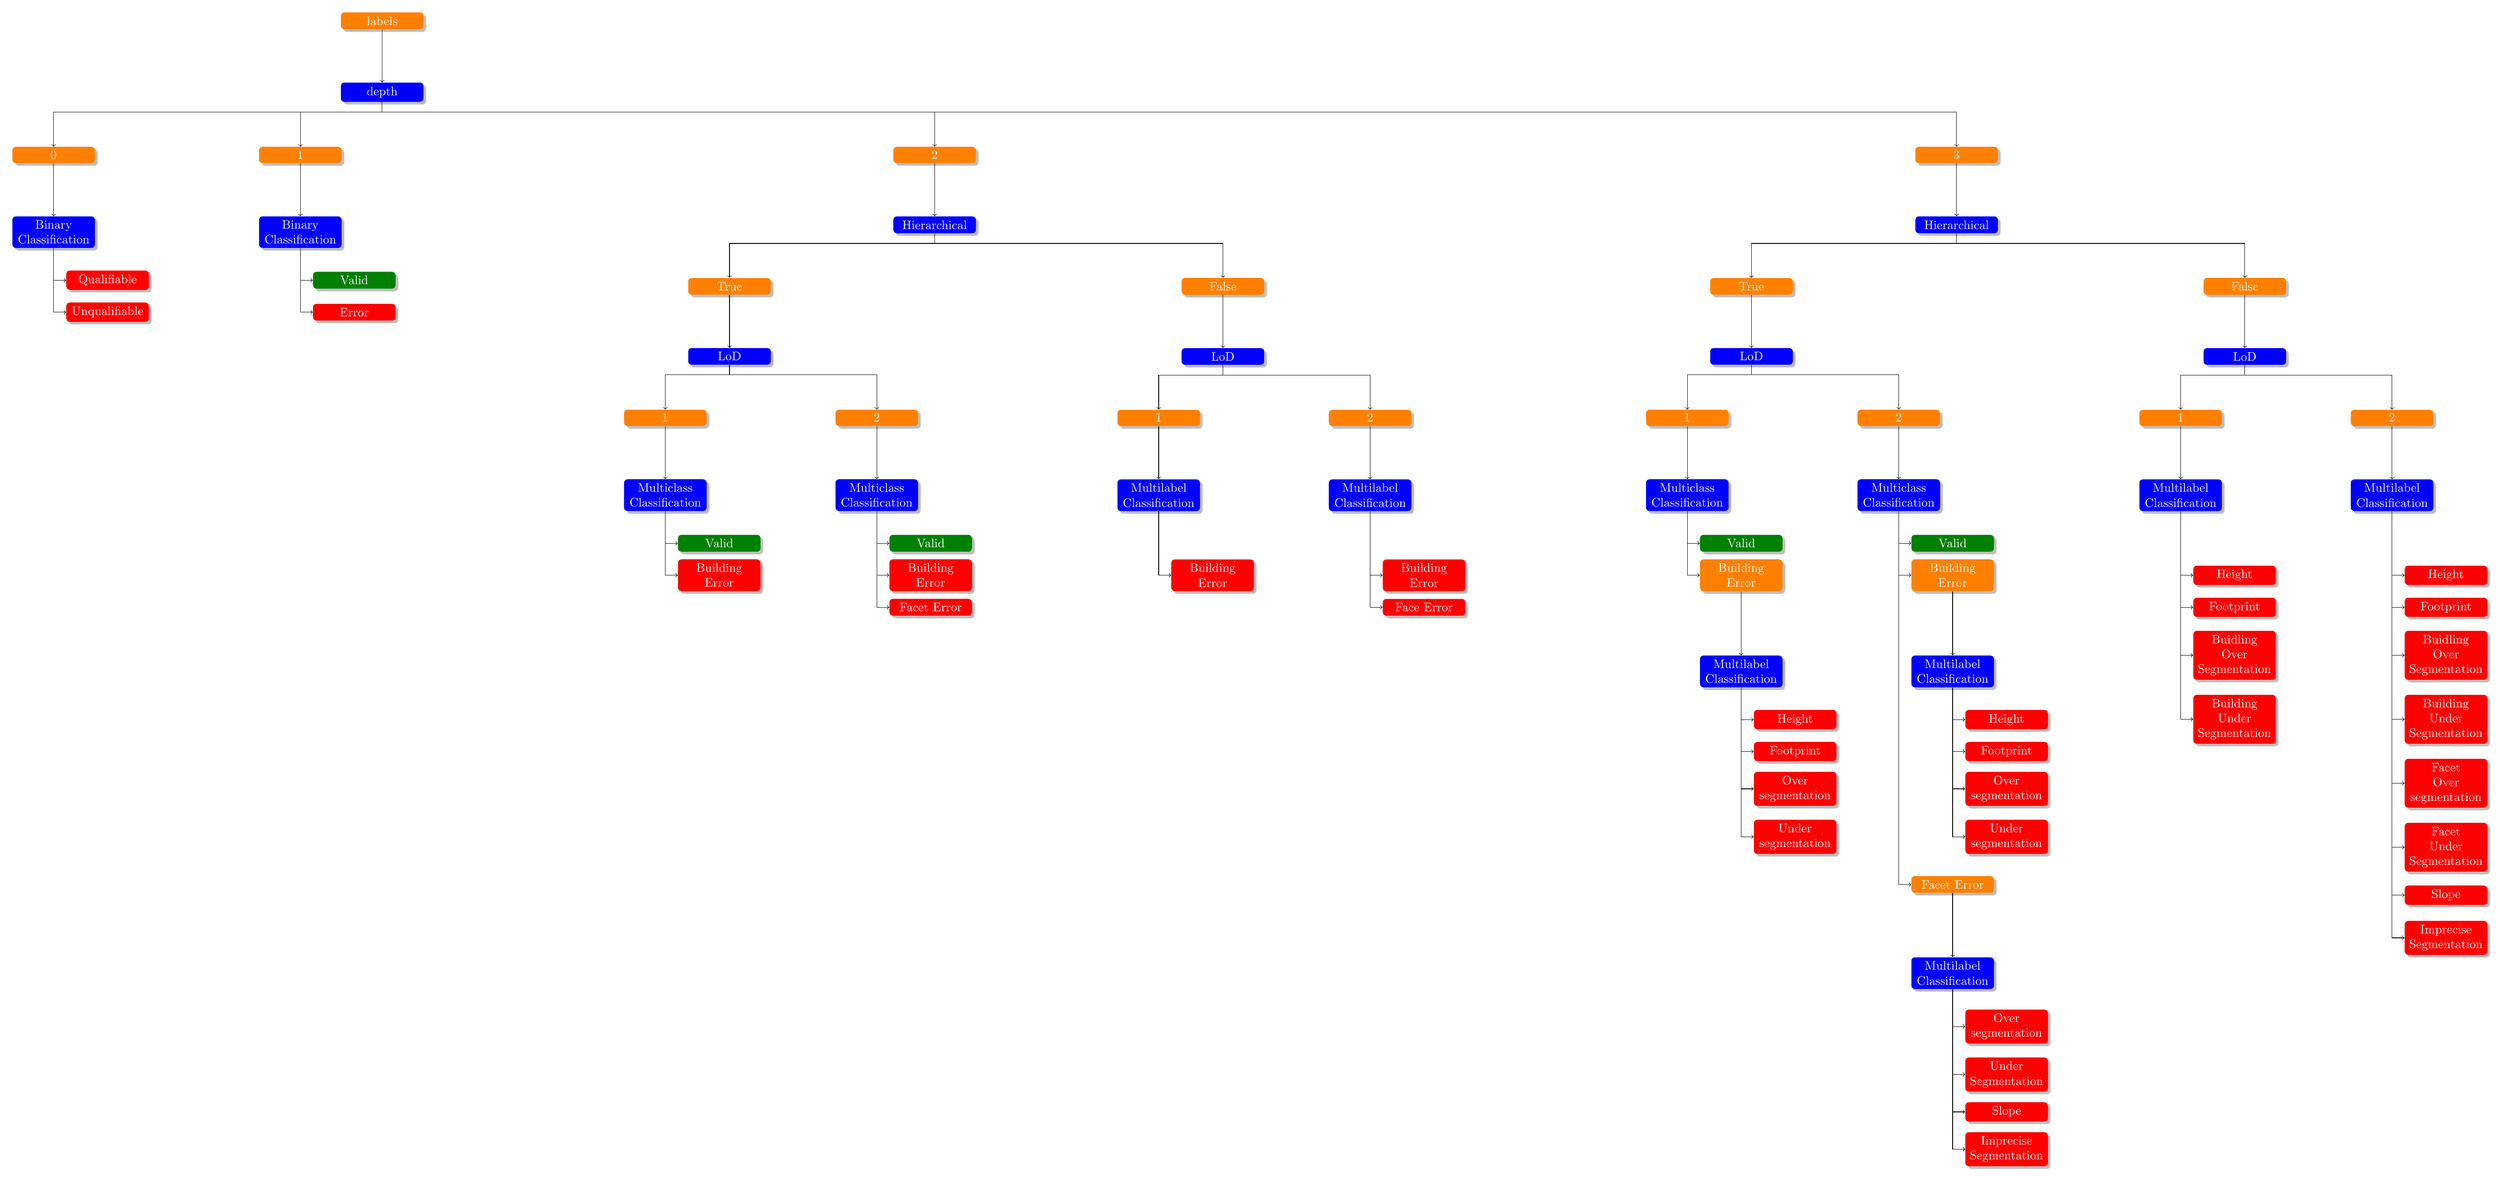
\begin{tikzpicture}[
        fork/.style={rectangle, draw=none, rounded corners=1mm, fill=blue, drop shadow,
            text centered, anchor=north, text=white, align=center, text width=6em},
        choice/.style={edge from parent path={(\tikzparentnode.south) -- +(0,-8pt) -| (\tikzchildnode.north)}},
        value/.style={rectangle, draw=none, rounded corners=1mm, fill=orange, drop shadow,
            text centered, anchor=west, text=white, text width=6em},
        classification/.style={grow=down, xshift=1em, edge from parent path={(\tikzparentnode.south) |- (\tikzchildnode.west)}},
        leaf/.style={rectangle, draw=none, fill=red, rounded corners=1mm, drop shadow,
            text centered, anchor=west, text=white, align=center, text width=6em},
        growth parent anchor=south,
        level 4/.style={sibling distance=14cm},
        level 6/.style={sibling distance=6cm}
    ]
	    \node (entry) [value] {labels} [->]
	        child{
	        node (depth) [fork] {depth}
	        child[choice, sibling distance=7cm]{
	            node (depth_0) [value] {$0$}
	            child[sibling distance=15cm]{
	                node (bin_class) [fork] {Binary\\Classification}
	                child[classification, level distance=6ex]{
	                    node (qual) [leaf] {Qualifiable}
	                }
	                child[classification, level distance=12ex]{
	                	node (unq) [leaf] {Unqualifiable}
	                }
	            }
	        }
	        child[choice, sibling distance=7cm]{
	        	node (depth_1) [value] {$1$}
	        	child{
	        		node (bin_class) [fork] {Binary\\Classification}
	        		child[classification, level distance=6ex]{
	        			node (qual) [leaf, color=black!50!green, text=white] {Valid}
	        		}
	        		child[classification, level distance=12ex]{
	        			node (unq) [leaf] {Error}
	        		}
	        	}
	        }
	        child[choice, sibling distance=29cm]{
	            node (depth_2) [value] {$2$}
	            child{
	                node (hier1) [fork] {Hierarchical}
	                child[choice]{
	                    node (1hier) [value] {True}
	                    child{
	                        node (1hierlod) [fork] {LoD}
	                        child[choice]{
	                            node (1hierlod1) [value] {$1$}
	                            child{
	                                node (1hiermulticl1) [fork] {Multiclass\\Classification}
	                                child[classification, level distance=6ex]{
	                                    node (1hierevalcl1) [leaf, color=black!50!green, text=white] {Valid}
	                                }
	                                child[classification, level distance=12ex]{
	                                	node (1hierebulcl1) [leaf] {Building Error}
	                                }
	                            }
	                        }
	                        child[choice]{
	                            node (1hierlod2) [value] {$2$}
	                            child{
	                                node (1hiermulticl2) [fork] {Multiclass\\Classification}
	                                child[classification, level distance=6ex]{
	                                    node (1hiervalcl2) [leaf, color=black!50!green, text=white] {Valid}
	                                }
	                                child[classification, level distance=12ex]{
	                                	node (1hierbulcl2) [leaf] {Building Error}
	                                }
	                                child[classification, level distance=18ex]{
	                                	node (1hierfaccl2) [leaf] {Facet Error}
	                                }
	                            }
	                        }
	                    }
	                }
	                child{
	                    node (1nonhier) [value] {False}
	                    child{
	                        node (1nonhierlod) [fork] {LoD}
	                        child[choice]{
	                            node (1nonhierlod1) [value] {$1$}
	                            child{
	                                node (1nonhiermultil1) [fork] {Multilabel\\Classification}
	                                child[classification, level distance=12ex]{
	                                	node (1nonhierbulcl1) [leaf] {Building Error}
	                                }
	                            }
	                        }
	                        child[choice]{
	                            node (1nonhierlod2) [value] {$2$}
	                            child{
	                                node (1nonhiermultil2) [fork] {Multilabel\\Classification}
	                                child[classification, level distance=12ex]{
	                                	node (1nonhierbulcl2) [leaf] {Building Error}
	                                }
	                                child[classification, level distance=18ex]{
	                                	node (1nonhierfaccl2) [leaf] {Face Error}
	                                }
	                            }
	                        }
	                    }
	                }
	            }
	        }
	        child[choice, sibling distance=29cm]{
	            node (depth_3) [value] {$3$}
	            child{
	                node (hier2) [fork] {Hierarchical}
	                child{
	                    node (2hier) [value] {True}
	                    child{
	                        node (2hierlod) [fork] {LoD}
	                        child{
	                            node (2hierlod1) [value] {$1$}
	                            child{
	                                node (2hiermulticl1) [fork] {Multiclass\\Classification}
	                                child[classification, level distance=6ex]{
	                                    node (2hiererrscl1) [leaf, color=black!50!green, text=white] {Valid}
	                                }
	                                child[classification, level distance=12ex]{
	                                    node (2hierbulcl1) [value] {Building Error}
	                                    child[choice]{
	                                        node (mlbulhier1) [fork] {Multilabel\\Classification}
	                                        child[classification, level distance=6ex]{
	                                            node (2hierbulcl1height) [leaf] {Height}
	                                        }
	                                        child[classification, level distance=12ex]{
	                                        	node (2hierbulcl1foot) [leaf] {Footprint}
	                                        }
                                            child[classification, level distance=19ex]{
	                                        	node (2hierbulcl1over) [leaf] {Over segmentation}
	                                        }
	                                        child[classification, level distance=28ex]{
	                                        	node (2hierbulcl1under) [leaf] {Under segmentation}
	                                        }
	                                    }
	                                }
	                            }
	                        }
	                        child{
	                            node (2hierlod2) [value] {$2$}
	                            child{
	                                node (2hiermulticl2) [fork, anchor=north] {Multiclass\\Classification}
	                                child[classification, level distance=6ex]{
	                                    node (2hiererrscl2) [leaf, color=black!50!green, text=white] {Valid}
	                                }
	                                child[classification, level distance=12ex]{
	                                    node (2hierbulcl2) [value] {Building Error}
	                                    child[choice]{
	                                        node (mlbulhier) [fork] {Multilabel\\Classification}
	                                        child[classification, level distance=6ex]{
	                                            node (2hierbulcl2height) [leaf] {Height}
	                                        }
	                                        child[classification, level distance=12ex]{
	                                        	node (2hierbulcl2foot) [leaf] {Footprint}
	                                        }
	                                        child[classification, level distance=19ex]{
	                                        	node (2hierbulcl2over) [leaf] {Over segmentation}
	                                        }
	                                        child[classification, level distance=28ex]{
	                                        	node (2hierbulcl2under) [leaf] {Under segmentation}
	                                        }
	                                    }
	                                }
	                                child[classification, level distance=70ex]{
	                                    node (2hierfaccl2) [value] {Facet Error}
	                                    child[choice, level distance=12ex]{
	                                        node (mlfachier) [fork] {Multilabel\\Classification}
	                                        child[classification, level distance=7ex]{
	                                            node (2hierfaccl2over) [leaf] {Over segmentation}
	                                        }
	                                        child[classification, level distance=16ex]{
	                                        	node (2hierfaccl2under) [leaf] {Under Segmentation}
	                                        }
	                                        child[classification, level distance=23ex]{
	                                        	node (2hierfaccl2slope) [leaf] {Slope}
	                                        }
	                                        child[classification, level distance=30ex]{
	                                        	node (2hierfaccl2impr) [leaf] {Imprecise Segmentation}
	                                        }
	                                    }
	                                }
	                            }
	                        }
	                    }
	                }
	                child{
	                    node (2nonhier) [value] {False}
	                    child{
	                        node (2nonhierlod) [fork] {LoD}
	                        child{
	                            node (2nonhierlod1) [value] {$1$}
	                            child{
	                                node (2nonhiermultil1) [fork] {Multilabel\\Classification}
	                                child[classification, level distance=12ex]{
	                                	node (2nonhierbulcl1height) [leaf] {Height}
	                                }
	                                child[classification, level distance=18ex]{
	                                	node (2nonhierbulcl1foot) [leaf] {Footprint}
	                                }
	                                child[classification, level distance=27ex]{
	                                	node (2nonhierbulcl1over) [leaf] {Buidling\\Over Segmentation}
	                                }
	                                child[classification, level distance=39ex]{
	                                	node (2nonhierbulcl1under) [leaf] {Building\\Under Segmentation}
	                                }
	                            }
	                        }
	                        child{
	                            node (2nonhierlod2) [value] {$2$}
	                            child{
	                                node (2nonhiermultil2) [fork] {Multilabel\\Classification}
	                                child[classification, level distance=12ex]{
	                                	node (2nonhierbulcl2height) [leaf] {Height}
	                                }
	                                child[classification, level distance=18ex]{
	                                	node (2nonhierbulcl2foot) [leaf] {Footprint}
	                                }
	                                child[classification, level distance=27ex]{
	                                	node (2nonhierbulcl2over) [leaf] {Buidling\\Over Segmentation}
	                                }
	                                child[classification, level distance=39ex]{
	                                	node (2nonhierbulcl2under) [leaf] {Building\\Under Segmentation}
	                                }
	                                child[classification, level distance=51ex]{
	                                	node (2nonhierfaccl2over) [leaf] {Facet\\Over segmentation}
	                                }
	                                child[classification, level distance=63ex]{
	                                	node (2nonhierfaccl2under) [leaf] {Facet\\Under Segmentation}
	                                }
	                                child[classification, level distance=72ex]{
	                                	node (2nonhierfaccl2slope) [leaf] {Slope}
	                                }
	                                child[classification, level distance=80ex]{
	                                	node (2nonhierfaccl2impr) [leaf] {Imprecise\\Segmentation}
	                                }
	                            }
	                        }
	                    }
	                }
	            }
	        }
	    };
    \end{tikzpicture}
\end{document}
